%%%----------------------------------------------------------
\chapter{Circle detection in binary dot images}
%%%----------------------------------------------------------

%Briefly state the task of this assignment in your own words (\ie, without reiterating the
%contents of the assignment sheet). Reference all literature, websites and other resources used,
%\eg, \cite{Higham1998,Guttman2001} or \cite{Mermin1989}. 
%The references are collected in a single section at the end of this document.

Detect a circle out that is embedded in a noisy binary image.

\section{Algorithm}
%TODO: Rewrite Algorithm Section

\begin{itemize}
	\item Collect the coordinates of all black pixels
	\item Randomly choose 3 points and use RANSAC Algorithm to detect points
	\item Calculate parameters of the circle (center point(x,y), radius) out of the 3 points
%TODO: Add Sources
%% Sources: 
%% https://math.stackexchange.com/questions/213658/get-the-equation-of-a-circle-when-given-3-points
%%https://math.stackexchange.com/questions/2836274/3-point-to-circle-and-get-radius?noredirect=1&lq=1
%% https://www.arndt-bruenner.de/mathe/scripts/kreis3p.htm
%% http://paulbourke.net/geometry/circlesphere/
	\item Count the points that are sufficiently close to the circle (certain distance parameter)
	\item Repeat the steps above and save the points of the best fitting circle (circle with highest point count)
	\item draw the circle onto the input image and output its parameters
\end{itemize}

\begin{figure}[htb]
	\centering
	\begin{minipage}[t]{0.49\linewidth}
		\centering
			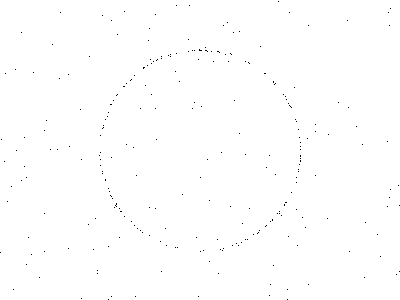
\includegraphics[width=.90\linewidth]{images/circle-test}
		\caption{Generated picture}
	\end{minipage}
	\hfill
	\begin{minipage}[t]{0.49\linewidth}
		\centering
		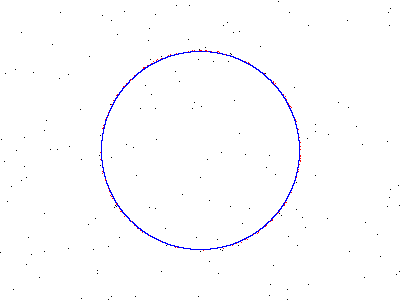
\includegraphics[width=.90\linewidth]{images/circle_result}
		\caption{Result picture}
	\end{minipage}
\end{figure}


%Geradengleichung aufstellen zwischen AB und BC - Mittelpunkt beider Geraden ermitteln - Normal Gerade durch den jeweiligen Mittelpunkt aufstellen und miteinander kreuzen -> Mittelpunkt 

\section{Research Question A}
\begin{itemize}
	\item The probability of selecting 3 circle points in a random draw if we make sure that we don't draw the same point twice is:
	\begin{displaymath}
	P = \frac{m}{n} \cdot \frac{m-1}{n-1} \cdot \frac{m-2}{n-2}
	\end{displaymath}
	\item There are at least 7 random draws needed to detect 3 circle points.
	\begin{eqnarray*}
	W = 1-(1-p)^n
	
	\end{eqnarray*}
\end{itemize}

%TODO: add to soruces
%https://www.mathe-online.at/materialien/Daniela.Eder/files/Diskrete_WK/Zusammenstellung.html

\section{Research Question B}

To detect multiple circles in one image we need to define a threshold for the number of points which are needed to be on a circle to be detected as a valid circle. If detected the circle is added to a list. To make sure that the same circle is not detected multiple times we need to check before adding it to the list that there is no circle with the same center point and radius already detected.